\begin{savequote}[9cm]
[...] we had to say it: “Okay, five Muslims were killed here, and five Christians were killed there.” So that there would be general consensus that there is a common enemy. 
\qauthor{--- Nigerian Journalist, November 2016}
\end{savequote}


\chapter[``Hey, They Aren't Muslims!'']{``Hey, They Aren't Muslims!''\footnote{This chapter is based on the following article: Demarest, L., Godefroidt, A., \& Langer, A. (2020). Understanding News Coverage of Religious-based Violence: Empirical and Theoretical Insights from Media Representations of Boko Haram in Nigeria. \textit{Journal of Communication}, Advance online publication: \href{https://academic.oup.com/joc/advance-article/doi/10.1093/joc/jqaa011/5841553}{https://doi.org/10.1093/joc/jqaa011}. I significantly contributed to this co-authored article---particularly to the theoretical framework advanced in the conclusion, the writing of the manuscript, and the code book used to collect the data---so that this article merits to be a chapter of my dissertation.}}
\chaptermark{Hey, They Aren't Muslims!}
\label{chap:chap4}


\begin{chapabstract}
Recent studies on conflict and terrorism news coverage have documented an in-group bias as well as an increasingly negative discourse about Muslims in the wake of Islamist terrorist attacks. Yet, as most of these studies have focused on Western media and settings, the determinants of news media’s religious biases and out-group categorizations remain insufficiently understood. In this chapter, we draw on interviews with Nigerian media practitioners and a comparison of Boko Haram news coverage in two Nigerian newspapers–-one Southern-based/Christian-affiliated and one Northern-based/Muslim-affiliated–-to argue that it is crucial to consider a country’s political-religious demography in order to understand the way in which religious-based violence is covered in the news. In this respect, we identify micro-, meso- and macro-level theoretical mechanisms through which a country’s demography can promote domestic news outlets–-regardless of their background and readership–-to cover conflict in a more balanced, nuanced, and objective way.
\end{chapabstract}
    

\newpage


%----------------------------------------------------------
\section{Introduction}
%----------------------------------------------------------

News media play a crucial role in keeping the public informed. Yet news outlets do not merely convey information, they also participate in the construction, maintenance, and transmission of particular narratives and discourses \citep[][p. 152]{Tenenboim-Weinblatt2016}. This becomes especially important in times of conflict, as narratives about the conflict may play a decisive role in influencing how people perceive the conflict, including its causes and consequences, and how policy-makers decide to deal with it \citep{Wolfsfeld2004}. Because of the immense societal importance of the way the media report on violence, it is hardly surprising that a large body of literature has emerged that analyses how political violence, violent conflicts, and terrorist attacks are being represented and framed in the media \citep[e.g.,][]{Baden2017, Baden2018, Gonen2019, Wolfsfeld2004}.


Arguably, the dominant paradigm in the study of conflict framing relates to the peace versus war journalism dichotomy \citep{Galtung1985, Galtung1998, Galtung2006}. `Peace journalism' focuses on the causes of conflict, the consequences for victims, and win-win conflict resolution. War journalism, in contrast, is more violence-, propaganda-, elite-, and victory-oriented, and treats conflict as an arena where participants are starkly grouped into opposing sides (`them vs. us') in a zero-sum game. While peace journalistic frames have shown to positively change audiences' empathy and understanding, albeit depending on individuals' prior beliefs and preconceptions, war journalism may negatively contribute to the conflict by focusing on violence, harsh military strategies, and the stark divide between in- and out-groups \citep{Kempf2017,McGoldrick2016}.


A large and growing number of studies has demonstrated that war-journalism frames dominate media depictions of political conflict \citep[][p. 152]{Tenenboim-Weinblatt2016}. Such war frames also appear particularly prevalent in Western media reporting of religious-based terrorism. Indeed, since the early 2000s, media outlets have increasingly reported in negative terms on Muslims following the spread of radical Islamist terrorism in Western societies \citep{Ahmed2017}.\footnote{In this chapter we use the terms Muslim and Islam to describe the broad category of followers of the Islamic religion. The term `Islamism' is used to denote the belief that Islam should order political society, with the additional connotation that violence can be used to fulfil this aim. Of course, the term `Islamism' has been contested and criticized, but it can be argued that our use of the term in this chapter closely fits the popular understanding of Islamism \citep[see][]{Martin2010}.} Rather than depicting extremists (i.e., the few people who commit or support religious-based violence and acts of terrorism) as the out-group, Western media have increasingly identified the Muslim community as a whole as `the other.' Such media narratives have not only contributed to a stronger in-group identification, but also increased out-group derogation and, thereby, strengthened `us versus them'-polarization \citep[e.g.,][]{Choma2015, dawson2011, Kteily2015a, Lopes2015}.


Yet, while media representations of Muslim minorities in times of terror have been widely studied in Western contexts, much less is known about how non-Western media construct and represent different religious groups in the wake of religious-based violence in their country. As a first step towards addressing this academic gap, we analyse media coverage of the Boko Haram insurgency in Nigeria, which emerged in the North-East of the country in 2002. Nigeria is a particularly interesting case for studying media representations of radical Islamist violence for a number of reasons. First, it is representative for the majority of cases of Islamist violence, which are, in fact, conducted in countries with a considerable share of Muslims and where many of the victims are Muslims themselves \citep{TheInstituteforEconomicsandPeace2016}. Second, as Muslims represent about half of the population, they are a politically influential and powerful group \citep{Mustapha2009, Nnoli1996}, in contrast to the marginalized minority groups they often constitute in Western societies. Third, similar to other African countries, the Nigerian media landscape suffers from a number of structural weaknesses which may impede professional reporting \citep{Frere2001}. It is in particular characterized by ethno-religious divides, with Christian-affiliated news outlets primarily based in the South of the country and Muslim-affiliated outlets in the North. These crucial differences in terms of religious-demographic structure, political power distribution, and characteristics of the media landscape, make Nigeria a powerful new case to study media representations of Islamist violence and Muslims, relative to Western cases. 

The research questions we specifically seek to address are: \textit{(1) How do Nigerian media report on the Boko Haram insurgency, and (2) how can we explain observed similarities and/or differences between Western and Nigerian media in terms of out-group representation of Muslims?} For our empirical analysis, we draw on interviews with Nigerian journalists and editors from different media houses across the North and the South of Nigeria, as well as a comparative content analysis of Boko Haram news coverage in two Nigerian newspapers---one from the Christian-majority South of the country (i.e., \textit{The Guardian}) and one from the Muslim-majority North (i.e., \textit{Daily Trust}). As such, we are able to analyze coverage of radical Islamist violence in a Muslim-majority context, as well as investigate whether reporting in a Christian-majority region follows Western media in their generally negative framing of Islam or not. %As we will show below, the Nigerian case does not only provide highly interesting empirical insights, but it is also a highly instructive theory-building case concerning the relationship between a country's religious-political demography and the way the media report on religious-based violence and terrorism. 


In what follows, we first discuss the literature on media representations of violent conflict, including religious-based terrorism, and highlight the relatively neglected dimension of media out-group categorization. Section \ref{sec:43} introduces the case of Nigeria. Here, we briefly outline the origins and evolution of the Boko Haram insurgency in the country as well as characteristics of the Nigerian media landscape. The latter is complemented with interview data with Nigerian media practitioners on religious bias in domestic news outlets. Section \ref{sec:44} then introduces the data and methodology used for our quantitative content analysis and presents our findings on how the Boko Haram insurgency has been framed and how media narratives are shaped by the societal actors given voice in reporting. Finally, in Section \ref{sec:45}, we build on these empirical insights by developing a novel theoretical model for explaining the relationship between a country's religious-political demography and the coverage of religious-based violence. 



%----------------------------------------------------------
\section{The Role of Media in Violent Conflict}
\label{sec:42}
%----------------------------------------------------------

Media scholars have long recognized that journalists do not simply relay facts, but also tend to include narratives that guide audience members' understanding of them. Framing theory \citep{Entman1993} serves as a useful lens to look at the communicative constitution of such narratives. Framing is defined as the process wherein news editors and journalists provide an interpretive structure for news facts by presenting information in a particular way \citep{Scheufele2014}. The resulting frames, or interpretative packages, are partly based on the (selected) perspectives of sources quoted and paraphrased in the news (i.e., the frame advocates). This process of selecting frames and frame advocates to convey and interpret information functions to ``promote a particular problem definition, causal interpretation, moral evaluation, and/or treatment recommendation'' of the events, issues, or actors being portrayed \citep[][p. 52]{Entman1993}. While media consumers do not blindly adopt these narratives, media framing can play an important role in how societal issues are understood and addressed \citep{Scheufele2014}. This is in particular the case for violent conflict. In times of conflict, news media may, for example, call for an aggressive military response or, conversely, propagate a more peaceful conflict resolution approach. Furthermore, the way the news is framed may also determine who the general public considers to be `the enemy' and `the victim'. As a result, news media may, both intentionally and unintentionally, fuel further tensions or promote reconciliation instead.


%----------------------------------------------------------
\subsection{The Peace Journalism Paradigm}
%----------------------------------------------------------
\cite{Galtung1985, Galtung1998, Galtung2006} was among the first to argue that media narratives on violent conflict can either entrench conflict or promote its resolution. He argued for the adoption of a particular style of conflict reporting termed `peace journalism'. Peace journalism aims to alter the conflict positively by nuancedly outlining the root causes of the conflict, seeking out constructive solutions and peacebuilding options, and avoiding divisive black and white terms. The opposite style is termed `war journalism' and has the danger to contribute negatively to the conflict by focusing on violence, military strategies, and winners and losers. 


While the war/peace journalism classification has remained the principal paradigm to study media reporting of violent conflict, it has also received substantial criticism, both on normative and scientific grounds. From a normative perspective there has been debate on whether peace journalism's advocacy for responsible journalism runs counter to the principle of objectivity \citep{Loyn2007, Lynch2007}. From a scientific perspective, a first criticism has focused on the dualistic nature of the peace versus war journalism paradigm. By introducing four alternative conflict news narratives, Teneboim-Weinblatt and colleagues (\citeyear{Tenenboim-Weinblatt2016}) have most recently argued against the dichotomous view on peace/war journalism and the idea that certain elements are clear indicators of one form of journalism over the other (e.g., elite/official actors as an indicator for war journalism). A second criticism has focused on the lack of attention for the various constraints that may shape the reality of conflict news production, including economic-organizational constraints \citep[such as the lack of resources, editorial hierarchies, and geographic absence/presence in the field; e.g.,][]{Hanitzsch2007, Hanitzsch2010, Wolfsfeld2004}, the agency of editors and journalists to select sources and transform available material into journalistic news frames \citep{Baden2018a}, and the larger socio-cultural context that form and limit the work of journalists \citep[e.g.,][]{Maslog2006, Zandberg2005}. In line with these criticisms, many scholars have recently shifted their attention from classifying media reports as war or peace journalism to the broader characteristics and determinants of media reporting on violent conflict.


%----------------------------------------------------------
\subsection{In-/Out-Group Construction in Conflict and Terrorism News}
%----------------------------------------------------------
One of the questions which has hereto received insufficient attention is how media narratives construct the groups involved in conflict in the first place. Peace journalism has always propagated overcoming `black-white', `good-bad', `us-them' binaries in conflict reporting, but has paid less attention to how media construct `us-them' group categories. While studies on political and media discourse have shown how in- and out-group categorization can take place \citep[e.g.,][]{Leudar2004, Sowinska2012, vanDijk2006}, we know less about the conditions under which certain groups are represented as out-groups. This is in particular the case for religious-based violence or terrorism. 


In this regard, an increasing number of studies has shown that in the aftermath of religious-based violence Western media have increasingly reported in negative terms on Muslims and have depicted the religion, instead of the few extremists who commit or support the violence, as `the threat' \citep{Ahmed2017}. The difference in labelling and framing of Islamist violence compared to other forms of political violence (e.g., white supremacist violence) is stark. \cite{Kearns2019}, for instance, report that violent attacks committed by Muslims receive, on average, over 357\% more media coverage than other attacks. This framing also impacts how people think about and categorize violence. The frequent use of the terrorist label by Western policymakers and media outlets to describe violent acts perpetrated by Muslims have led citizens to equally label acts of violence more often as terrorism when carried out by a Muslim and less when they are carried out by whites or individuals with a history of mental illness \citep{DOrazio2018, Huff2018}.


Yet, as the paragraph above demonstrates, our knowledge on conflict framing in general and terrorism news in particular is largely built on a Western field of study. This is an important remark because the vast majority of past studies rests on the assumption that in- and out-groups are clearly separated, with Muslims often being the religious minority in the country of study. Indeed, communication scientists have repeatedly highlighted an in-group, one-sided, and ethnocentric bias inherent in news reporting in general \citep{Gans1980} and, particularly, in conflict and terrorism coverage \citep{Galtung1965, Wolfsfeld2008}. Yet in order to contribute to the broader theoretical question of the factors influencing such in- and out-group identification and bias in the media, it is necessary to investigate conflict reporting in a more diverse body of cases, characterized by a more diverse composition of ethnic and/or religious groups \citep[see also][p. 236-237]{Ahmed2017}. For instance, we know less about how news outlets report on religious-based violence in a country where Muslims do not constitute a small and marginalized minority. The framing of the Boko Haram crisis in Nigeria, we argue, is therefore an important case to that aim as it concerns radical Islamist violence in such an under-researched context.


%----------------------------------------------------------
\section{Nigeria as an Instructive Case-Study (Part II)}
\label{sec:43}
%----------------------------------------------------------
Nigeria is a highly ethnically and religiously diverse country. Some estimates put the number of ethnic groups in Nigeria at about 250 \citep[][pp. 5-6]{Graf1988}. However, the three major ethnic groups are the Hausa-Fulani in the North, the Igbo in the South-East, and the Yoruba in the South-West. In terms of religion, Islam is widely practised in the North, while traditional religions and Christianity characterize the South. In contrast to Western societies, Christians and Muslims are largely similar in size, both constituting about half of the population. Importantly, ever since the amalgamation of Northern and Southern Nigeria in 1914, ethno-regional tensions have been pervasive and have repeatedly led to conflict \citep{Suberu2001}. The emergence of the radical Islamic movement, Boko Haram, has further strained inter-religious relations in Nigeria in recent years. 


In what follows, we first briefly outline the Boko Haram insurgency. Next, we describe some of the main characteristics of the Nigerian media landscape. To do so, we also draw on in-depth interviews conducted with Nigerian journalists and editors on the media coverage of the insurgency to highlight the contrasting perceptions on media content between practitioners themselves. This leads to our own content analysis in Section \ref{sec:44}.


%----------------------------------------------------------
\subsection{The Boko Haram Insurgency}
\label{sec:431}
%----------------------------------------------------------
There is ongoing debate on the origin of the Boko Haram movement, but it is generally believed that the sect emerged around the mid-1990s in North-Eastern Nigeria and flourished under various names before it named itself \textit{Jamā'at Ahl Al-Sunna Li-L-Da'Wa Wa-L-Jihād} (i.e., people committed to the propagation of the prophet's teachings and jihad) and became widely known as ``Boko Haram'' (i.e., Western education is forbidden) \citep{Mustapha2014b}. The professed objective of the group was the strict implementation of Sharia law in Nigeria \citep{Onuoha2015}. The sect regularly came into conflict with authorities since its emergence, but the violence escalated after the July 2009 uprisings in Borno state \citep{Mustapha2014b}.


Since 2009, the Boko Haram insurgency has claimed about 20,000 lives, led to over two million displaced citizens, and caused severe infrastructure destruction and economic loss \citep{GCT2018}. After the infamous April 14 2014 Chibok girls kidnapping, Boko Haram grew stronger and was able to conquer substantial parts of territory in the North-East of Nigeria. In the run-up to the 2015 elections, incumbent president Goodluck Jonathan initiated a multinational task force and eventually succeeded in reclaiming most territory before the elections. Winner of the elections, president Muhammadu Buhari, carried this \'{e}lan further throughout 2015 when the crisis seemed to be dissipating. Recently, however, the group has claimed new kidnappings, attacks, and suicide bombings, taking again hundreds of lives \citep{AmnestyInternational2018}. 


At first the insurgency in North-Eastern Nigeria seemed to target Christian enclaves in the North-East, which led to the narrative that Boko Haram was a Muslim initiative aimed at annihilating Nigerian Christians \citep{PerousedeMontclos2015}. But moderate Muslims quickly became victims to the sect's violence as well, stimulating discussion on the root causes of the insurgency. These root causes can be found, among other things, in the socio-economic marginalization of the Northern states \citep{Langer2017c}. Nonetheless, political elites have also played a role in the escalation of the Boko Haram crisis as it is said that the group was first recruited and armed by politicians and abandoned after election time \citep[][p. 227]{Kendhammer2016}, and as poor governance and repressive state policies escalated the crisis into violence \citep[][see also Appendix \ref{app:A2}]{Mustapha2014b, PerousedeMontclos2015}.


%----------------------------------------------------------
\subsection{The Nigerian Media and Religious-Based Violence}
\label{sec:432}
%----------------------------------------------------------
Nigerian media are known to be among the most vibrant and critical in Sub-Saharan Africa \citep{FreedomHouse2017}. Yet similar to other African countries, Nigerian media suffer from a number of structural weaknesses which may impede professional reporting, including a lack of resources to conduct independent reporting, proper training, and capacity-building opportunities \citep{Frere2001}. Low journalist wages can also give rise to corruption or `brown envelope' journalism \citep{Lodamo2009}. These structural constraints may contribute to divisive and nefarious reporting by creating dependencies on powerful actors such as the government and political parties. This has led several authors to raise concerns on political biases in Nigerian media \citep[e.g.,][]{Ette2018}.


Attention to possible religious bias in Nigerian news media has most recently come to the fore with the emergence of violent interreligious conflict in Central Nigeria and the Boko Haram crisis. Based on qualitative discourse analysis, \cite{Musa2013} argue that Southern papers mostly depict Christians as victims and Muslims as perpetrators in religious riots in Central Nigeria, while Northern papers do the reverse. By investigating the language of report headlines, \cite{Yushau2015} argues that during the beginning of the Boko Haram uprising in 2009, a Northern newspaper (i.e., \textit{Daily Trust}) used more moderate headlines when reporting on the group than a Southern paper (i.e., \textit{The Guardian}) did. The Southern newspaper also appeared more likely to link the group to Islam and Muslims in general. By contrast, more recent quantitative research suggests that while Nigerian newspapers tend to have political affiliations, this does not necessarily skew their reporting on political violence \citep{Demarest2018}. Furthermore, while Nigerian news media do not address the political and economic root causes of violent conflict, at the same time, they do not attribute violence to ethnic and religious differences as such \citep{Demarest2019}. These studies hence shed a more positive light on Nigerian media practices. 


Moreover, Nigerian media editors and journalists themselves are divided as to whether ethno-regional positions and ownership structures affect conflict reporting. As part of this study, we conducted in-depth interviews with representatives of various newspapers, radio stations, and television outlets on ethno-religious biases in news media and the representation of the Boko Haram crisis in particular. Interviews took place in Abuja (the Northern official capital) and Lagos (the Southern economic capital) in November 2016 and in December 2017. Respondents were recruited using a snowball sampling technique. In total, 26 participants were interviewed. This sample includes both Christians/Southerners and Muslims/Northerners.\footnote{For more information about respondents and their news outlets, please see Table \ref{tab:art3-app-tab1} in Appendix D.} 


A first finding from the interviews was that many media practitioners recognized that ownership structures and a lack of resources constrain reporting: ``The ownership of some of the papers and media houses; who are they!? They come from a Christian faith or a Muslim faith. Whether I like it or not, they have an interest and that interest you must also capture'' (Journalist, Voice of Nigeria, November 2016); ``Most media houses don't pay salaries. If you are not paid, of course, you compromise with stories from people with interests. Who pays? Political parties, religious groups etc. ({\dots}). These things can trigger crisis'' (Editor, National Mirror, December 2017). 


According to some journalists, these issues had implications for reporting: ``Daily Trust is mostly established with a Northern and Muslim agenda. What they report mostly are things that are sympathetic to the Northern Muslims'' (Member, Nigerian Union of Journalists (NUJ), November 2016). Yet others countered this idea: ``Daily Trust mostly has a Northern readership, but they are careful not to be seen as a Muslim voice. They also seek balance. It's not an Islamic paper'' (Editor, News Diary, November 2016); ``Religion and region are there, but not enough to affect the viewpoint'' (Editor, The Guardian, December 2017).


When it comes to the reporting of the Boko Haram crisis, some argued that Muslim journalists and outlets were (more) actively involved in defending Islam as such: ``Media houses owned by Muslims try to more or less moderate their language.'' (Editor, Authority, December 2017). Or: 

\begin{quote}
Us, Muslim journalists, report events as they unfold. Their [Boko Haram] strategy was to create disruption and confusion between Muslims and Christians, so we tried to stop this, for example by reporting their Islamic writings on a wall were not correct (Editor, News Agency of Nigeria, December 2017). 

Sometimes professionally, you don't need to tell the faith of somebody, so that you not aggravate counter-attack somewhere. But we realized that at a certain level we had to say it. ``Okay, five Muslims were killed here, and five Christians were killed there.'' So that there would be general consensus that there is a common enemy (Journalist, Daily Trust, November 2016).
\end{quote}


Many Southern-based/Christian journalists stressed similar tactics, however, and argued that they also defended Islam: ``We try to educate people [that] Islam is not as portrayed, it is not what people see from the Boko Haram crisis. We report from the true practices of Islam. We have a diverse team here with Christians and Muslims'' (Editor, The Guardian, December 2017); or ``When reporting on Boko Haram, we use terms such as insurgents or extremist. We try not to talk about Islam. We live together with Christians and Muslims'' (Editor, The Nation, November 2017).


As touched upon above, the case of Nigeria is instructive because it allows us to systematically analyse news coverage of radical Islamist violence in a non-Western country where Muslims are not a minority. As the above paragraphs suggest, however, investigating Boko Haram coverage in Nigerian media is also important because media practitioners themselves are divided on how the insurgency has been represented, and in particular whether there are divisions between Northern and Southern news outlets. Building on the views found in our interview data, we hence conducted a quantitative content analysis of two Nigerian newspapers which have their origin in different parts of the country.


%----------------------------------------------------------
\section{Boko Haram in \textit{The Guardian} and \textit{Daily Trust}}
\label{sec:44}
%----------------------------------------------------------
%----------------------------------------------------------
\subsection{Data}
\label{sec:441}
%----------------------------------------------------------
For our quantitative content analysis, we selected \textit{The Guardian} and \textit{Daily Trust} newspapers. While more newspapers originate from the South of the country, \textit{The Guardian} is among the most well-known and has been used in previous research that compares Northern and Southern reporting \citep{Ette2018, Yushau2015}. \textit{Daily Trust}, on the other hand, is the most established Northern newspaper. Both \textit{The Guardian} and \textit{Daily Trust} circulate in the North and South of Nigeria, but primarily in larger urban centres.\footnote{Only 23,25\% of Nigerians read the newspaper a few times a week or more, but research shows that especially educated elites, to which policymakers tend to belong, rely on newspapers as their source of information regarding what is going on in the country (Afrobarometer, 2014).} For both newspapers, we were able to obtain digital copies of newspaper issues. As sampling frame, we selected news reports in-between April 2014 and March 2015 because this was the period when Boko Haram was able to conquer substantial parts of the North-East before being pushed back in the run-up to the March 2015 elections. We randomly select one report on Boko Haram per issue during this period and hence acquire a representative sample of reports for both newspapers. Reports were sampled based on the key term `Boko Haram', by consequence reports which used this term more frequently had a higher chance of being selected. In our analyses, we control for word length to partially compensate for the fact that longer reports were more likely to be selected. Reports which focused more strongly on Boko Haram were also more likely to be selected, but we do not consider it likely that this biases the sample. We included regular news reports as well as editorials, opinion pieces, interviews, reports from foreign sources (e.g., the Economist)\footnote{\cite{Wahutu2018a} points out that in violent conflict reporting African media often rely on international news wires, which has implications for studying African media representations themselves. In the case of the domestic Boko Haram crisis, international news wire services were sometimes relied on, but this remained limited overall.}, and others (e.g., print versions of speeches delivered on events). 

In total, we coded 711 news reports, 349 from \textit{The Guardian} and 362 from \textit{Daily Trust.}\footnote{Both newspapers publish issues on Sunday, but not on a small number of selected holidays. Several issues of \textit{The Guardian} could also not be obtained. The missing issues are spread well over the one-year period.} For every article we noted the date, page number, word length, and type of report. For our coding scheme we drew on Entman's general framework (\citeyear[][p. 52]{Entman1993}) distinguishing between the framing of causes, consequences, and solutions. The specific frames corresponding to these three categories were themselves established by drawing on the literature on peace journalism \citep[e.g.,][]{Shinar2009}, the academic literature on the Boko Haram crisis and its root causes (see Section \ref{sec:431}), and our interview data (see Section \ref{sec:432}). 


First, for the causal frames, we distinguished between socio-economic, political, and religious framing. Following the peace journalism literature, socio-economic and political causes can be considered as root causes of a conflict and, by using these frames to explain the crisis, media may reduce societal tensions and promote the search for conflict resolution. The framing of Boko Haram as driven by religion and particularly Islam, by contrast, can fuel inter-group tensions. The issue of whether Boko Haram has been religiously framed in Nigeria has also been prominently debated by our interviewees, with some explicitly stating they take up a defending role towards Islam (see Section \ref{sec:432}). To measure the extent to which the Boko Haram insurgency has been religiously framed in general, we measure the mentioning of religious causes (e.g., radicalization, Islamism, al-majiri\footnote{Al-majiri are students of Islamic education, which takes place outside of the formal schooling system. In Northern Nigeria, al-majiri are commonly associated with poverty as many parents send their children to Islamic schools because they are unable to provide for them. In certain Islamic schools (but certainly not all), al-majiri may be exposed to radical Islamism. Furthermore, they also tend to be vulnerable to abuse and mistreatment.}) as well as whether religious causes are explicitly rejected (e.g., `Boko Haram has nothing to do with Islam'). The established causal frames hence allow us to analyse whether news outlets differ in the way they represent the most prominently debated causes of the Boko Haram crisis.\footnote{Some news articles and interviewees also referred to external causes of the Boko Haram crisis, including the Libyan conflict and the roles of Cameroon and Chad in supporting Boko Haram. We chose not to code this information as an external causes frame because it does not provide us more insight into the use of peace journalistic practices.}


Second, with respect to the consequences of Boko Haram, we assessed to what extent different societal costs were mentioned. Attention to the suffering of victims can be considered peace journalistic because it can create support for peacebuilding. More specifically, we focused on human costs (casualties), economic costs (infrastructure destroyed, loss of livelihoods), and psychological costs (trauma, feelings such as hopelessness, fear, distrust). While all three are negative consequences, the latter may be considered particularly peace journalistic because it focuses on the less visible effects of violence, while the more visible ones may engender calls for further violence and retribution \citep{Shinar2009}. We also focus on victim labels, in particular mentions of their religious identity. The initial targeting of Christians by Boko Haram (see Section \ref{sec:431}) still raises debates on who the principal victim of the crisis is, even if the violence in the North-East has escalated to the extent that Muslims make up the majority of the victims. The extent to which media emphasize the religious identity of the victims was also a major concern for several interviewees (see Section \ref{sec:432}). By coding victims' religion where mentioned, we are able to check whether \textit{The Guardian} is more likely to stress `own' Christian victims, or vice versa for \textit{Daily Trust}. Stressing victims on only one side of a conflict may fuel further tensions according to the peace journalism literature. For the case of Boko Haram, it may in particular risk creating the perception of wider societal conflict between Christians and Muslims.


Last, with respect to the proposed solutions, we coded whether socio-economic measures (e.g., job creation), diplomatic measures (e.g., negotiations, reintegration programmes), and/or militaristic solutions (e.g., more security, better intelligence, more weapons) were suggested by the news outlets. Militaristic solutions may be considered as tending towards war journalism, while the mentioning of socio-economic and diplomatic measures can rather be considered peace journalism. We did not find evidence of a potential religious dimension in the treatment recommendation for the crisis in the literature and our interview data, hence we only focus on these general peace journalistic categories.


Besides the framing of causes, consequences, and solutions, we also investigated whether articles criticized or defended the federal government's response to the crisis in order to further assess possible political-regional bias. Given that the Southern politician Goodluck Jonathan was president during this period, we could expect \textit{The Guardian} to defend the federal government's actions if their reporting is influenced by region of origin. In the same vein, \textit{Daily Trust} would criticize the federal government as Jonathan's major challenger for the 2015 elections was the Muslim Northerner Muhammadu Buhari. Specific attention was also devoted to the semantics used to describe Boko Haram in reporting. We coded whether the article used language referring to the religious nature of Boko Haram (leaving aside the group name itself), and whether Boko Haram were referred to as criminal actors. This allows us to investigate whether \textit{The Guardian} is more likely to depict Boko Haram in a religious manner, and whether \textit{Daily Trust} is more likely to use criminalizing language. Finally, we coded the presence of frame advocates that were quoted or paraphrased in the article as this allows us to investigate how the inclusion of certain sources influences a report's general narrative. Building on Tenenboim-Weinblatt and colleagues (\citeyear{Tenenboim-Weinblatt2016}), we coded different types of elite actors including politicians, security officials, civil society, and religious actors. In addition, we included Boko Haram itself as a frame actor as well as the public (eyewitnesses, bystanders, and victims). 


All variables were coded as binary with 0 indicating `not mentioned' and 1 indicating `mentioned'. This decision was taken from an agenda-setting perspective as we are interested in whether certain causes were mentioned at all or rather kept out of the news. There are two exceptions here. First, while our variable on religious causes takes on the value of 1 when such causes were mentioned, an additional variable measures whether an article explicitly rejected the view that Islam was a cause of the Boko Haram crisis. When this view was rejected, the variable takes on the value of 1; if it was not rejected, the value equals 0. Second, the government response variable is measured on a 5-point scale ranging from very negative (0) to very positive (4). 


Two coders pretested the coding scheme independently, discussed questions, and changed the codebook when deemed necessary. This pilot allowed for a more careful tailoring of our variables to debates and discursive practices in Nigerian reporting. The full dataset was coded by a principal coder, while the second coder recoded a subset of the sample ($N=31$ for \textit{Daily Trust} and $N=30$ for \textit{The Guardian}) to check intercoder reliability coefficients. Krippendorff alphas ranged between .82 and 1 which indicates excellent intercoder reliability \citep{Krippendorff2018}. The sampling protocol and codebook are available in Appendix \ref{app:D2}, whereas the dataset and syntax are available as \href{https://academic.oup.com/joc/article/70/4/548/5841553#supplementary-data}{online appendices}.

%----------------------------------------------------------
\newpage
\subsection{Findings}
\label{sec:442}
%----------------------------------------------------------

\subsubsection{Boko Haram in \textit{The Guardian} and \textit{Daily Trust}}
In this section, we investigate how Nigerian media represent the Boko Haram crisis and whether there are differences between \textit{The Guardian} and \textit{Daily Trust}. First, it is important to note that there are some significant differences between the newspapers concerning the coverage allocated to the Boko Haram uprising as such. On average, \textit{The Guardian }counts more pages (\textit{M} = 77.61, \textit{SE} = 0.75) than \textit{Daily Trust} (\textit{M} = 64.81, \textit{SE }= 0.44), and articles on Boko Haram have a higher word count in \textit{The Guardian} (\textit{M} = 1168.65, \textit{SE} = 45.13) than in \textit{Daily Trust} (\textit{M} = 772.36, \textit{SE} = 40.90). Both differences in length are significant, $t(565.502) = -14,90, p < .001$ and $t(699.498) = -6.51, p < .001$ respectively. Still, \textit{The Guardian} does refer less---and not more---to the Boko Haram crisis per issue (\textit{M} = 19.23, \textit{SE }= 0.75) than \textit{Daily Trust} (\textit{M} = 28.90, \textit{SE }= 0.97), $t(672.213) = 7.904, p < .001$). Of course, this finding is related to the fact that readers from \textit{Daily Trust} are more likely to be affected by the Boko Haram insurgency.


Besides differences in length, there are also some differences between the newspapers concerning the types of reports included in the sample. \textit{The Guardian }published more standard news reports ($\chi^2 = 3.96, p = .047$) and more interviews ($\chi^2= 6.17, p =.013$), whereas \textit{Daily Trust} published more foreign articles ($\chi^2 = 22.10, p < .001$). Since the length and type of the report might affect its framing, we controlled for word count and type of report when comparing the framing of the Boko Haram conflict in \textit{The Guardian }and \textit{Daily Trust} via logistic regression analyses. The report control variable is a dichotomous indicator for standard reports versus others as the latter are generally more sensitive to subjective narratives. Furthermore, \textit{Daily Trust} is always taken as reference category (see Table \ref{tab:art3-tab1} on the next page for all results).


The descriptive statistics in Table \ref{tab:art3-tab1} (see columns `Total', `Guardian', and `\textit{Daily Trust}') indicate that both newspapers devote relatively similar levels of attention to each of the frames and frame actors. With regard to the causes, we find that the socio-economic causes of the Boko Haram crisis are least likely to be mentioned by both media outlets, even though these are arguably most often stressed in the literature \citep[e.g.,][]{Langer2017c, PerousedeMontclos2015, Mustapha2014b}. Political causes are mentioned more frequently, similar to religious causes. Nevertheless, while religious causes are cited frequently, it occurs often that the role of religion in instigating the crisis itself is refuted. Notably, refuting religion as a root cause of the conflict is even more likely than the mentioning of socio-economic causes. 
\newpage

%---------------------------------
% Table 1
%---------------------------------
\begin{table}[H]
\caption{Framing Boko Haram in\textit{ The Guardian} (=1) versus \textit{Daily Trust} (=0)}
\label{tab:art3-tab1}
\small
\onehalfspacing
\begin{threeparttable}
\resizebox{\textwidth}{!}{%
\begin{tabular}{@{}llccccc@{}}
\toprule
\multicolumn{2}{l}{Variables} &
  \begin{tabular}[c]{@{}c@{}}Total\\(N=711)\end{tabular} &
  \begin{tabular}[c]{@{}c@{}}Guardian\\(N=349)\end{tabular} &
  \begin{tabular}[c]{@{}c@{}}Daily Trust\\(N=362)\end{tabular} &
  $\chi^2$ &
  Odds ratio\tnote{a} \\ \midrule
\multicolumn{2}{l}{Causes}       &         &         &         &           &          \\
     & Socio-economic            & 8.02\%  & 10.89\% & 5.25\%  & 7.664\textsuperscript{**}   & 1.787    \\
     & Political                 & 18.00\% & 22.35\% & 13.81\% & 8.774\textsuperscript{**}   & 1.898\textsuperscript{**}  \\
     & Religion                  & 17.58\% & 20.92\% & 14.36\% & 5.265\textsuperscript{*}    & 1.247    \\
     & Religion not a cause      & 9.42\%  & 12.32\% & 6.63\%  & 6.743\textsuperscript{**}   & 1.868\textsuperscript{*}   \\ 
\multicolumn{2}{l}{Consequences} &         &         &         &           &          \\
     & Socio-economic            & 30.52\% & 31.81\% & 29.28\% & 0.534     & 0.798    \\
     & Human                     & 69.06\% & 72.78\% & 65.47\% & 4.443\textsuperscript{*}    & 1.130    \\
     & Psychological             & 23.91\% & 23.78\% & 24.03\% & 0.006     & 0.783    \\
     & Christian victims         & 12.94\% & 15.19\% & 10.77\% & 3.071     & 1.227    \\
     & Muslim victims            & 20.25\% & 18.62\% & 21.82\% & 1.126     & 0.638\textsuperscript{*}   \\
\multicolumn{2}{l}{Solutions}    &         &         &         &           &          \\
     & Socio-economic            & 3.66\%  & 5.44\%  & 1.93\%  & 6.215\textsuperscript{*}    & 2.385    \\
     & Diplomacy                 & 16.60\% & 17.77\% & 15.47\% & 0.676     & 1.039    \\
     & Military                  & 39.10\% & 43.55\% & 34.81\% & 5.709\textsuperscript{*}    & 1.216    \\
     & Government evaluation     & 1.71    & 1.79    & 1.62    & -2.330\textsuperscript{*}   & 0.143\tnote{b}   \\
\multicolumn{2}{l}{Semantics}    &         &         &         &           &          \\
     & Islam                     & 27.57\% & 31.81\% & 23.48\% & 6.167\textsuperscript{*}    & 1.286    \\
     & Crime                     & 9.00\%  & 13.18\% & 4.97\%  & 14.615\textsuperscript{***} & 2.700\textsuperscript{**}  \\
\multicolumn{2}{l}{Actors}       &         &         &         &           &          \\
     & Political leaders         & 42.05\% & 41.26\% & 42.82\% & 0.177     & 0.827    \\
     & Security personnel        & 25.18\% & 23.50\% & 26.80\% & 1.027     & 0.622\textsuperscript{*}   \\
     & Christian authorities     & 8.30\%  & 12.89\% & 3.87\%  & 19.026\textsuperscript{***} & 3.287\textsuperscript{***} \\
     & Muslim authorities        & 8.16\%  & 8.88\%  & 7.46\%  & 0.481     & 1.057    \\
     & Civil society             & 19.13\% & 22.06\% & 16.30\% & 3.817     & 1.180    \\
     & Public                    & 20.96\% & 16.91\% & 24.86\% & 6.791\textsuperscript{**}   & 0.419\textsuperscript{***} \\
     & Boko Haram                & 12.38\% & 10.32\% & 14.36\% & 2.687     & 0.527\textsuperscript{**}  \\ \bottomrule
\end{tabular}}
\begin{tablenotes}
\vspace{-5mm}
\singlespacing
\footnotesize
\item[a] Results from logistic regression analyses controlling for word count and report type
\item[b] t-statistic instead of $\chi^2$; unstandardized OLS regression coefficient instead of odds ratio, controlled for word count and report type. \\ \textsuperscript{*}\(p<0.05\), \textsuperscript{**}\(p<0.01\), \textsuperscript{***}\(p<0.001\).
\end{tablenotes}
\end{threeparttable}
\end{table}
\newpage

Controlled for length and type of report we only find significant differences between both newspapers for the political cause variable, and for the variable indicating whether reports explicitly rejected the view that Boko Haram is related to Islam. Both variables are more likely to be mentioned in \textit{The Guardian}. This means that the view that a Southern-based newspaper would be less likely to report on root causes and would link the insurgency to religion is not supported. This finding is corroborated by the fact that there is no significant difference between both newspapers in their references to Islamic radicalization as a cause of the crisis.\footnote{We also tested whether there was a difference between both newspapers with regard to the mentioning of religious causes, without explicit denial. A new variable was created to test this based on the existing ones. No significant differences emerged from our analyses ($\chi^2$-test and logistic regression).}


The consequences of the Boko Haram crisis receive more attention in both newspapers than the causes of the crisis, especially the socio-economic and human costs, and to a lesser extent the psychological costs. No significant differences are found for these variables between the outlets---even though northern Nigeria has been more affected by Boko Haram violence. Furthermore, religious identification of victims is not as frequent as the mentioning of the costs of the conflict as such, yet still relatively frequent. While it appears that the proportion of Christian victims mentioned is higher for \textit{The Guardian} than \textit{Daily Trust}, this is not significant. Muslim victims do appear more likely to be mentioned in \textit{Daily Trust}, after controlling for word count and report type. Nevertheless, for both newspapers the percentage of Muslim victims mentioned is higher than that for Christian victims, which is in line with the facts on the ground. In general, the evidence suggests that neither of the newspapers propagates the belief that Boko Haram is a Muslim sect striving to annihilate Christians specifically.


No significant differences exist between the newspapers with regard to the solution frames. Both \textit{The Guardian} and \textit{Daily Trust} devote most attention to security-based solutions. Soft approaches involving diplomacy and reconciliation are mentioned far less often than hard approaches. In line with the scant attention paid to the socio-economic cause of the crisis, least attention is devoted to long-term development to address the uprising. It is also interesting that while \textit{Daily Trust} appeared significantly more likely to be critical of the federal government, this difference disappears after controlling for length and type of report. Hence, \textit{The Guardian} does not take up a defending role vis-a-vis Southern president Goodluck Jonathan. Indeed, in both newspapers most reports have a negative stance towards the federal government. 


Regarding the semantics, we find that the religious labelling of the group occurs frequently, and that this holds for both newspapers. This labelling actually occurs more often than the mentioning of religious causes as such. We find that \textit{The Guardian} is slightly more likely to give a religious label to Boko Haram, yet this difference fails to reach statistical significance after controlling for length and report type. \textit{The Guardian} is, however, more likely to use criminalizing labels than \textit{Daily Trust}. Overall, criminal labels are used less frequently than religious ones. In line with our findings on the reporting of the causes of the crisis, we find that the Southern-based newspaper does not appear to link Boko Haram to Islam in general.


For both \textit{The Guardian} and \textit{Daily Trust }political leaders and security personnel are the dominant frame actors in Boko Haram reporting. Security actors are somewhat more likely to be included in \textit{Daily Trust}, however, controlled for word length and report type. A starker significant difference is found with regard to the inclusion of Christian authorities, which are a lot more prominent in \textit{The Guardian} than \textit{Daily Trust}. No differences are found for Muslim authorities. The voices of public witnesses tend to be included quite often as well, but relatively more so by \textit{Daily Trust}. This could be explained by the fact that \textit{Daily Trust }as a Northern newspaper is more closely located to the conflict and has therefore more access to people on the ground. The Northern newspaper also included Boko Haram more often as a frame actor than \textit{The Guardian}. In the following section, we analyse to what extent the voices included in media reporting influence the representation of the crisis.


\subsubsection{Frame Advocates and Narratives}

While our previous comparison did not reveal sharp differences between \textit{The Guardian} and \textit{Daily Trust} newspapers, we also investigate to what extent certain actors (i.e., frame advocates) are associated with the causes, consequences, and solutions mentioned in newspaper articles as well as the semantics used. This gives us further insight in how societal actors themselves (attempt to) shape conflict narratives. Logistic regression analyses are used to test for the impact of actors on frames used, with each frame as dependent variable and the actor categories, word count, type or report, and \textit{Daily Trust} as independent variables (see Table \ref{tab:art3-tab2}).

\newpage
\begin{table}[H]
\begin{adjustwidth}{-0.1in}{-0.2in} % adjust the L and R margins
\caption{Actor Inclusion and the Media Representation of the Boko Haram Crisis}
\label{tab:art3-tab2}
\onehalfspacing
\small
\begin{tabular}{@{}llccccccccc@{}}
\toprule
          &                   & \multicolumn{4}{c}{Causes}         & \multicolumn{5}{c}{Consequences}                \\ \cmidrule(l){3-11} 
\multicolumn{2}{l}{}          & SE   & Pol.   & Rel.    & Not Rel. & SE      & Hum     & Psych   & CV      & MV      \\ \midrule
\multicolumn{2}{l}{Actors}    &      &        &         &          &         &         &         &         &         \\
          & Political         & .88  & 1.98\textsuperscript{**} & .91     & 1.47     & 1.45\textsuperscript{*}   & 1.48\textsuperscript{*}   & 1.57\textsuperscript{*}   & .94     & 1.20    \\
          & Security          & 1.19 & .69    & 1.18    & .93      & 1.31    & 1.38    & 1.22    & .56     & 1.03    \\
          & Christian         & 1.04 & .62    & 1.62    & 1.60     & 1.22    & 1.57    & 1.84    & 4.82\textsuperscript{***} & 2.34\textsuperscript{*}   \\
          & Muslim            & 1.30 & .67    & 2.59\textsuperscript{**}  & 9.94\textsuperscript{***}  & 1.59    & 1.99    & 2.81\textsuperscript{**}  & 1.37    & 3.91\textsuperscript{***} \\
          & CSO               & 1.93 & 1.55   & 1.32    & .88      & 1.07    & 1.81*   & 1.21    & 1.28    & .56\textsuperscript{*}    \\
          & Public            & .59  & .62    & 1.56    & .81      & 3.47\textsuperscript{***} & 5.05\textsuperscript{***} & 4.17\textsuperscript{***} & 4.44\textsuperscript{***} & 5.89\textsuperscript{***} \\
          & BH                & 1.46 & 1.62   & 3.32\textsuperscript{***} & 1.29     & 1.25    & 2.86\textsuperscript{**}  & 1.26    & 1.58    & 1.80\textsuperscript{*}   \\
\multicolumn{2}{l}{Newspaper} &      &        &         &          &         &         &         &         &         \\
          & Guardian          & 1.80 & 2.08\textsuperscript{**} & 1.49    & 1.86\textsuperscript{*}    & 0.99    & 1.40    & 0.93    & 1.35    & 0.78   \\*\bottomrule
\end{tabular}
\end{adjustwidth}
\end{table}

\addtocounter{table}{-1}

\begin{table}[H]
\caption*{Table 4.2 continued ... }
\onehalfspacing
\small
\begin{tabular}{@{}lL{2.2cm}L{1.5cm}p{1.5cm}p{1.5cm}p{1.5cm}p{1.5cm}p{1.5cm}@{}}
\toprule
          &                   & \multicolumn{4}{c}{Solutions}       & \multicolumn{2}{c}{Semantics} \\\cmidrule(l){3-8} 
\multicolumn{2}{l}{}          & SE     & Dipl.   & Mil.    & Govt\textsuperscript{a}   & Islam          & Crime        \\ \midrule
\multicolumn{2}{l}{Actors}    &        &         &         &        &                &              \\
          & Political         & .91    & 2.53\textsuperscript{***} & 1.74\textsuperscript{**}  & .07    & 1.278          & 1.363        \\
          & Security          & 1.87   & .72     & 2.61\textsuperscript{***} & -.06   & .829           & 1.814        \\
          & Christian         & 1.07   & 2.62\textsuperscript{**}  & 1.15    & -.18   & 1.317          & 1.650        \\
          & Muslim            & 3.21   & 1.87    & 1.72    & .10    & 3.268\textsuperscript{***}       & 3.422\textsuperscript{**}      \\
          & CSO               & 4.21\textsuperscript{**} & 1.79    & 1.34    & -.05   & 1.632\textsuperscript{*}         & 1.925        \\
          & Public            & .16    & .65     & .49\textsuperscript{**}   & -.30\textsuperscript{**} & 1.911\textsuperscript{*}         & .459         \\
          & BH                & 1.37   & 3.98\textsuperscript{***} & 1.14    & -.11   & 3.507\textsuperscript{***}       & 1.186        \\
\multicolumn{2}{l}{Newspaper} &        &         &         &        &                &              \\
          & Guardian          & 2.34   & 1.06    & 1.25    & 0.11   & 1.557\textsuperscript{*}         & 2.721\textsuperscript{**} \\*\bottomrule    
\end{tabular}
\vspace{-5mm}
\singlespacing
\footnotesize
\textit{Note:} SE=Socio-Economic, Pol.=Political, Rel.=Religion, Not Rel.= Religion explicitly rejected as cause, Hum.=Humanitarian, Psych=Psychological, CV=Christian Victims, MV=Muslim Victims, Dipl.=Diplomacy, Mil.=Military, Govt.=Government response evaluation; CSO=Civil society organization. Reported results are odds ratios from logistic regressions controlling for word count and report type, with \textsuperscript{*}\(p<0.05\), \textsuperscript{**}\(p<0.01\), \textsuperscript{***}\(p<0.001\); with the exception of \textsuperscript{a} which are OLS regression, unstandardized coefficient.\par
\end{table}

\newpage


The frame advocates used in the article can only partly explain the mentioned causes. Political causes are related more to the discourse of political authorities, who often attempt to discredit political opponents by accusing them of fuelling the crisis. Civil society organization are more likely to be associated with socio-economic causes. Especially international NGOs (e.g., International Crisis Group, \textit{Daily Trust} 5 April) and academic actors (e.g., Wole Soyinka, \textit{Daily Trust} 12 April) were likely to mention socio-economic causes of the conflict. The mentioning of religious causes does not appear to be related to the inclusion of Christian authorities, but it is highly related to the inclusion of Muslim authorities. Muslim authorities are more likely to mention Islam as a cause of the Boko Haram crisis, but predominantly to counter this view as can be seen from the odds ratio for the variable indicating that a report explicitly rejects that Boko Haram is caused by Islam. Lastly, Boko Haram's own discourse also revolves around religion as a cause. Indeed, the group, and especially its leader Abubakar Shekau, rarely mention socio-economic and political grievances, but state their goals in terms of a radicalized Islamist ideology. The group's own narratives hence preclude an identification of deeper underlying causes, which can have implications for policy-making to end the crisis, in particular through diplomatic means. It is also important to note that, even after controlling for the impact of selecting frame advocates, \textit{The} \textit{Guardian} remains more likely than \textit{Daily Trust} to actively counter the discourse that the crisis is driven by religion.


While the religious-regional affiliation of the newspapers did not affect which consequences were mentioned, the inclusion of specific actors does affect the mentioned consequences. Political actors, for instance, are associated with all three consequences as they often express sympathy for the suffering of civilians in their discourses. The inclusion of religious authorities also increases the likelihood that psychological and human consequences will be mentioned, but it also increases the risk of in-group bias. While Christian authorities are more likely to stress Christian victims, Muslim authorities are more likely to acknowledge Muslim victims. Importantly, controlling for the actors included renders the previously found difference between \textit{The Guardian }and \textit{Daily Trust} with regard to the inclusion of Muslim victims insignificant. While both newspapers do not differ in the inclusion of Muslim authorities, \textit{Daily Trust} does include more witnesses and victims (i.e., the public), which are often Muslim. This is potentially due to the closer proximity to the conflict.


Turning to the solutions, civil society actors are significantly related to the mentioning of socio-economic solutions. For civil society actors this is in line with their mentioning of socio-economic causes. Diplomacy as the second soft approach is significantly related to political and Christian authorities. Boko Haram is also positively associated with the mentioning of a diplomatic solution. This association is mostly driven by reports focusing on the Chibok girls. Some reports detail how Boko Haram's leadership has boasted about the capture of the girls and how other actors call for negotiations to bring the girls back. Other reports focus on Boko Haram's offer of a swap deal for the return of the girls, which ultimately did not take place. It is not the case, however, that Boko Haram has called for peace negotiations and amnesty as such. Political and security actors are associated with the mentioning of military solutions. The public is the only actor that significantly increases the odds of government criticism. As citizens experience daily attacks, their testimonies are often accompanied by statements on the lack of security in their home region and how they are abandoned by security personnel when attacks occur. 


With regard to the semantics, we find that Muslim authorities are more likely to refer to the religious nature of Boko Haram, but this can be explained by the fact that they mostly counter the view that Islam is associated with the group's violence. Moreover, Muslim authorities are also the only actors associated with the criminal labelling of the group. Interestingly, Christian authorities do not appear to be associated with the religious labelling of Boko Haram, while this does appear to be the case for civil society actors and the public. Clearly, Boko Haram also increases the likelihood of religious labels, in line with our findings on religion as a cause of the crisis. 

What is particularly interesting from these analyses is that while the Boko Haram crisis is in itself strongly debated by different societal actors both \textit{The Guardian} and \textit{Daily Trust} include them in such a way as to represent the conflict relatively similarly. This is specifically the case for the more potentially divisive actors such as politicians and religious authorities. Neither newspaper allows itself to become associated with a certain political stance by including politicians from different backgrounds. While the inclusion of Muslim and Christian authorities risks in-group bias with regard to the religious identification of victims, this did not affect the overall stance of both papers. The president of the Christian Association of Nigeria (CAN) was once quoted in \textit{The Guardian} as saying: ``As far as we are concerned, it is a war against Christians and Christianity'' (\textit{The Guardian}, 3 May), but such narratives did not dominate the Southern newspaper.


%----------------------------------------------------------
\newpage
\section{Theoretical Discussion and Conclusion}
\label{sec:45}
%----------------------------------------------------------

While the instrumental role of the media in shaping people's perceptions concerning the causes and dynamics of religious-based violence has been widely studied in Western societies (e.g., Baden, 2014; Tenenboim-Weinblatt, Hanitzsch \& Nagar, 2016; Wolfsfeld, 2004), much less is known about this important issue in non-Western settings. The current chapter aims to contribute towards filling this important academic gap by analysing media coverage of the Boko Haram insurgency in Nigeria. More specifically, we aimed to answer the following research questions: \textit{(1) How do Nigerian media report on the Boko Haram insurgency, and (2) how can we explain observed similarities and/or differences between Western and Nigerian media in terms of out-group representation of Muslims? }


With respect to the first research question, our empirical analysis has shown that Nigerian newspapers generally adopted a war-oriented narrative rather than a peace journalistic approach by, first, highlighting the (visible) consequences of violence rather than their root causes and, second, urging for military solutions instead of propagating peaceful conflict resolution approaches. This pattern is in line with Western studies on conflict news coverage (e.g., Baden \& Tenenboim-Weinblatt, 2018a) and reflects broader news values and journalist routines that structure the news (Galtung \& Ruge, 1965; Gans, 1980; Harcup \& O'Neill, 2001). Yet, in contrast to most Western studies on conflict news coverage (e.g., Ahmed \& Matthes, 2017), our empirical analysis also showed that Nigerian newspapers generally did not associate Boko Haram's violent insurgency with Islam and Muslims as such. This finding is important because it indicates that, even in a context where tensions between religious groups have repeatedly led to conflict and media may be susceptible to political influences due to resource deficits, one religion is not necessarily associated with the violence perpetrated by a small sub-group claiming to act in the name of that religion.


Interestingly, the absence of an association between Boko Haram and Islam was true for the Northern-based (and, hence, Muslim-affiliated) newspaper and the Southern-based (and, hence, Christian-affiliated) newspaper alike. Overall, the two newspapers reported in very similar ways on the Boko Haram crisis---again arguing against the often-assumed in-group, one-sided, and ethnocentric bias inherent in news reporting in general (Gans, 1980) and, particularly, in conflict and terrorism coverage (Galtung \& Ruge, 1965; Wolfsfeld et al., 2008). Even the few differences in who was quoted or cited (e.g., the Southern-based newspaper relied more often on Christian authorities, whereas the Northern-based newspaper had more access to security actors and witnesses) did not translate into sharp differences in what was reported.  The lack of a systematic association between Boko Haram and Islam constitutes an important difference with Western media coverage of religious-based violence and relates to our second research question, that is, understanding and explaining the differences between Western and Nigerian media in terms of out-group representation of Muslims within a context of religious-based violence. 


In order to explain these differences, we argue that it is crucial to consider countries' political-religious demography. More specifically, we theorize that the extent to which religious groups in a particular society are represented, both demographically and politically, influences the extent to which (1) day-to-day interactions and contact take place between individuals from these different groups, (2) certain norms and practices of inter-religious understanding enter the newsroom, and (3) individuals from different religious groups hold powerful political positions. These three mechanisms, in turn, can stimulate domestic news outlets---regardless of their background and readership---to cover conflict in a more balanced, nuanced, and objective way. The proposed theoretical mechanisms linking a country's political-religious demography to the nature of its media coverage of religious-based conflict are visualised in Figure \ref{fig:art3-fig1}.


%~~~~~~~~~~~~~~~~~~~~~~~~~~~~~~~~~~~
% Figure 1
%~~~~~~~~~~~~~~~~~~~~~~~~~~~~~~~~~~~
\vspace{3mm}
\begin{figure}[H]
\centering
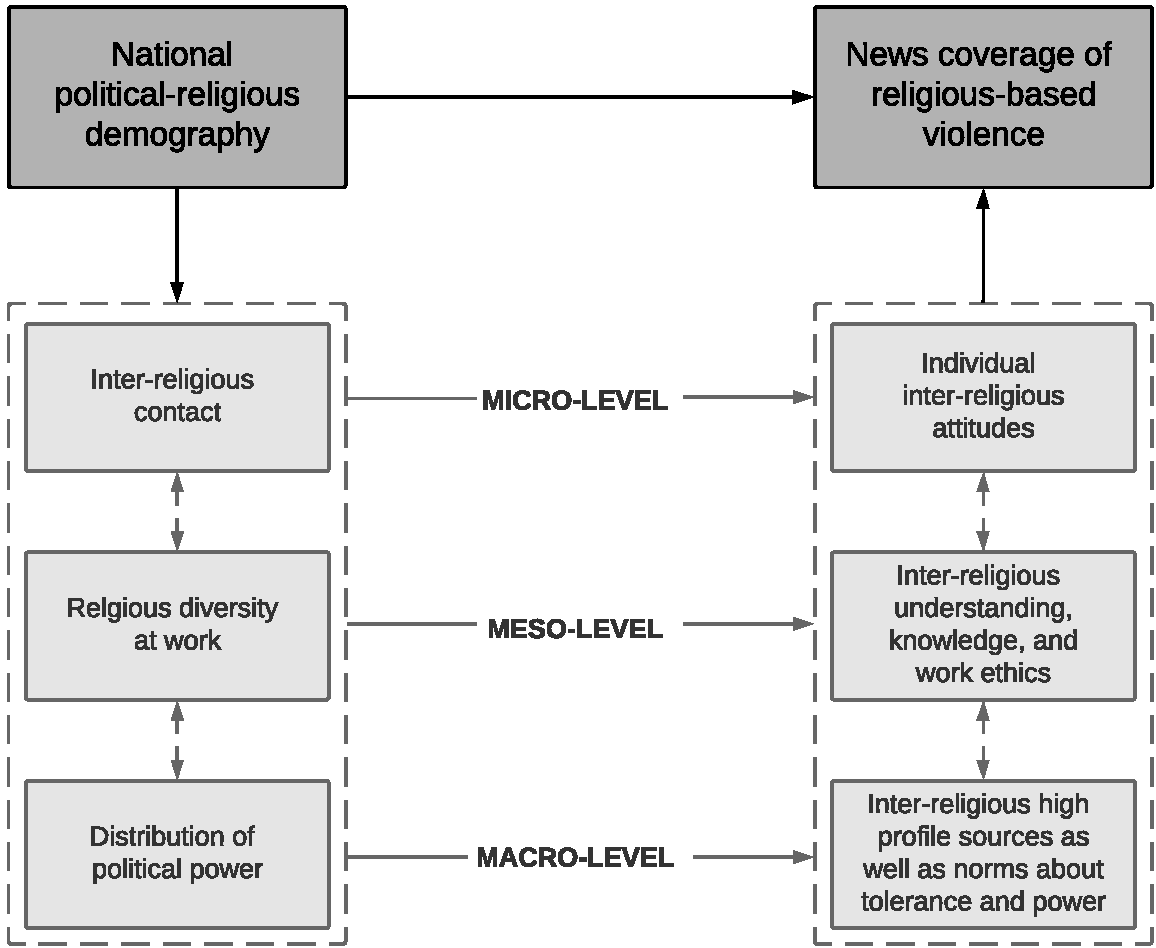
\includegraphics[width=0.8\textwidth]{Chapter_4/art3-figure1.pdf}
\caption{Theoretical Model Explaining News Coverage of Religious-Based Violence}
\label{fig:art3-fig1}    
\end{figure}
%~~~~~~~~~~~~~~~~~~~~~~~~~~~~~~~~~~~
\newpage


In what follows, we briefly outline our micro-, meso-, and macro-level mechanisms to explain differences in how Western and non-Western news outlets report political violence and, particularly, radical Islamist violence. 


First, our proposed micro-level mechanism builds upon the well-known intergroup contact theory \citep{Pettigrew2006, Pettigrew2008a}. In countries where Muslims and Christians both constitute a substantial proportion of the population, there are more opportunities for intergroup contact compared to countries where Muslims represent only a small minority of the population (as is the case in most Western countries). Indeed, many Muslims and Christians in Nigeria interact on a daily basis, and inter-religious friendships and marriages are common. Out-group attitudes---including those of journalists, editors, and news sources---are thought to be more tolerant and less prejudiced following positive intergroup contact. This, in turn, may be reflected in the way media report about radical religious-based violence. In addition, inter-religious contact can also guard against out-group categorization in a more direct way because it increases access to sources across religious lines \citep[see also][]{Gonen2019}. This access can facilitate the likelihood that Christians see and hear that ordinary Muslims do not support jihadism and realize that all Nigerians---regardless of their religious background---are a victim of the violence. This idea of ``we're all in this together'' is illustrated by one of our respondents saying that ``[{\dots}] it was not all about Muslims killing Christians but certain fundamentalists killing both Muslims and Christians for not agreeing with what they want to propagate'' (Journalist, Daily Trust, November 2016). 



Second, our proposed meso-level mechanism focuses on the composition of and subsequent norms and practices within the professional environment. Again, the composition of groups in a society is likely to be reflected in the composition of the workplace---including media houses and publication outlets. This idea is mentioned as well by one of our interviewees emphasizing that they ``have a diverse team here with Christians and Muslims'' (Editor, The Guardian, December 2017). The presence and collaboration of representatives of both religious groups within professional media is thought to positively impact the way these media report religious-based violence. Muslim journalists, for example, may act as ``watchdogs'' \citep[see][p. 254]{Nishikawa2009}, deliberately pointing out stories that are not sufficiently nuanced and/or indirectly sensitizing their Christian colleagues. This meso-level causal mechanism is also supported by \cite{Bunce2010}, for instance, who suggested that diversity in Kenyan newsrooms guards against divisive reporting. \cite{Gonen2019} also demonstrated how interactions between journalists across conflict lines helps to gather more accurate information and to understand the conflict in a more comprehensive way. The argument is also in line with findings that gender balance \citep[e.g.,][]{Shor2019} and minority inclusion \citep[e.g.,][]{Johnston2007, Nishikawa2009} in the workplace may bring unique perspectives to the table and reshape journalistic norms and practices. Yet, the latter studies have equally emphasized remaining obstacles hampering the positive impact of a diverse newsroom, especially real-world structural inequalities and lack of minorities in power positions \citep{Johnston2007, Nishikawa2009}---an important factor which brings us to our third and last mechanism. 


Last, our proposed macro-level mechanism touches upon the distribution of power between groups at the national level. In Nigeria, since independence, both Muslims and Christians have held powerful positions, including those of military ruler and president, and various other institutional mechanisms have been put in place to safeguard religious balance at several decision-making levels \citep[e.g.,][]{Mustapha2009}. This power distribution can impact news coverage in several ways. First, political power may directly translate into news coverage given news media's focus on elite sources \citep{Gans1980}. Indeed, as Hopmann, de Vreese and Albaek (\citeyear[][pp. 276-277]{Hopmann2011}) put it: ``The more powerful you are, the more attention you receive.'' As Muslims constitute an important share of Nigeria's elite, both Christian- and Muslim-based news outlets give Muslim elites voice in reporting as frame advocates (see also Table \ref{tab:art3-tab1} for empirical evidence of this argument). These are then able to challenge negative stereotyping of Islam and produce counter-narratives. Second, political power can also be used to shape press laws and media policies. In Nigeria, relatively stringent press laws were introduced under military rule to prevent ethno-religious hate speech, and many remain in place today \citep{Demarest2018}. These laws were implemented by Christian and Muslim power-holders to protect Nigerian unity, and can be used by both sides to constrain media discourse. This may lead to more cautious journalists and editors in reporting religious-based violence. Third and last, while press laws have been implemented to protect Nigerian unity by means of coercion, it is also possible that over time the norm of unity and equal representation has been internalized by media practitioners and society as a whole. As a result, Muslim journalists in Nigeria may also enjoy a greater ability to question certain media practices because they are more supported by these institutionalized norms. Hence, differences between the prevailing power structures in Western and non-Western contexts are important to take into account as well when studying how news media report on group-based violence. 
\newpage


In conclusion, by unravelling a predominantly war-oriented coverage of the Boko Haram insurgency in Nigerian newspapers, our findings corroborate the general patterns in conflict journalism outlined by the peace journalism framework. But, by highlighting important differences between Nigerian and Western media in the out-group categorization of Muslims, we also drew attention to the dynamics of group categorization and its determinants. We suggested that a country’s political-religious demography is an important explanatory factor for media out-group categorization. Our findings on the representation of radical Islamist violence may hold for other countries where Muslims form a sizeable group in the population, including those on West-Africa’s coastal line, but further research is needed to fully unravel how different religious compositions may lead to different media representations and to deductively test our proposed mechanisms. In addition, it remains important to also keep into account that demography is only one aspect, while political power is another, especially given that some countries provide more political power to religious minorities than others (e.g., Lebanon). Finally, while we have focused in this theoretical discussion on the presence and position of certain groups in a society, other situational or contextual factors (such as the exact type of conflict under examination and its corresponding fault lines, its intensity/saliency, and/or conflict (a)symmetry) may equally warrant further investigation.

%%%%%%%%%%%%%%%%%%%%%%%%%%%%%%%%%%%%%%%%%%%%%%%%%%
% Keep the following \cleardoublepage at the end of this file, 
% otherwise \includeonly includes empty pages.
\cleardoublepage
